%!TEX root = ../thesis.tex
\section{Implementation}\label{sec:implementation}
\subsection{Used Tools, Frameworks and Libraries}
\Cref{tab:usedTools} lists all tools, frameworks and libraries \drivebuild{} uses, characterizes them by whether the \gls{mainapp}, a \gls{simnode} or a client implementation requires them and shows whether they are just a dependency of another element.
This section describes the most essential tools, frameworks and libraries in detail and why they were chosen.\\
\beamng{}~\cite{beamNG} is a racing game that is free to use for research purposes.
It comes with a highly accurate physics engine and thus it is interesting for research as well.
Most simulators have a top down approach where the physics of a vehicle are specified as a whole and the properties and behavior of all components of the car derive from it.
In contrast \beamng{} uses a bottom up approach where each tire, car suspension, the chassis, the engine, every cross beam, \etc{} has its own physics.
A vehicle is a collection of these components which are connected by beams and thus the physics the vehicle results from the physics of its components.\\
\beamngpy{}~\cite{beamngpy} is a Python interface for \beamng{}.
It allows to programmatically create scenarios, attach many kinds of sensors to vehicles, collect data and handle simulations and participants during simulations.
\beamngpy{} can also access the pixel perfect annotation mode in which a camera returns images that mark on the image where buildings, roads, other participants \etc{} are.
This can be used to gather training data for \glspl{ai}.
Since \beamngpy{} is not able to handle parallel requests to the same \beamng{} instance \drivebuild{} wraps \beamngpy{} and introduces locks to implement basic thread safety.\\
\dill{} is a library which can serialize Python objects and extends the capabilities of the \pickle{} module that ships with Python.
\glspl{simnode} have to serialize parameters when a process starts a new thread \eg{} start a new \beamng{} instance and requires arguments.\\
\flask{}~\cite{flask} is a framework to create micro service based webservices.
It is well known, reliable and uses annotations to map addresses with functions and parameters which makes it easy to use.\\
\lxml{}~\cite{lxml} is a library for handling \gls{html} and \gls{xml} files.
It provides methods to parse and validate \gls{xml} files against \glspl{xsd} and to traverse them with XPath expressions.
\lxml{} is basically just a Python interface to the well known, reliable and very fast C libraries libxml2~\cite{libxml2} and libxslt~\cite{libxslt}.\\
\Gls{protobuf}~\cite{protobuf} is a tool to specify and handle messages in a more type safe way than basic byte streams offer.
Therefore it provides a language to define the structure of messages and the data types of their attributes.
\Gls{protobuf} is able to cross compile these definitions to appropriate representations in a set of well known programming languages including Python, Java, C++ and Haskell.
The compilation process introduces additional methods to serialize and parse messages and to check the existence of attributes in messages.\\
\winpython{}~\cite{winpython} is a Python distribution that ships with a set of Python packages for which the installation on Windows is complex or error prone.
This includes especially packages like \scipy{} which \drivebuild{} requires.
\subsection{Communication}\label{subsec:communication}
Both the content of \gls{http} requests as well as of socket messages is serialized byte data which represents \glspl{pmessage}.
The communication uses the generated serialization methods of \Gls{protobuf} to convert \glspl{pmessage} from and to byte data.
\Cref{fig:simpleMessages} lists all simple and \cref{fig:complexMessages} visualizes all complex \glspl{pmessage} which the communication can handle as well as their structure.
\begin{figure}
    \centering
    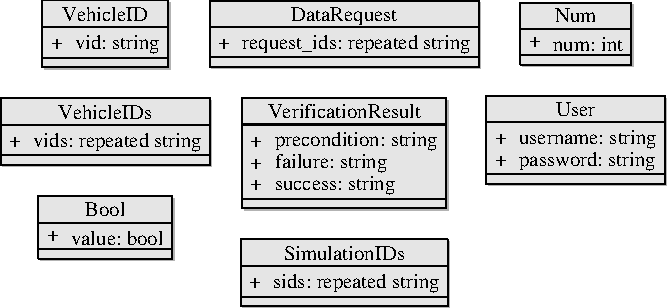
\includegraphics[width=\textwidth, height=.95\textheight, keepaspectratio]{diagrams/messagesTypeGraph-1.pdf}
    \medskip
    \caption{%
        Simple \glspl{pmessage} --- Shows all basic \glspl{pmessage} which do neither contain nor are nested in other \glspl{pmessage}.
        It also lists their attributes with the appropriate type.
    }\label{fig:simpleMessages}
\end{figure}
\begin{figure}
    \centering
    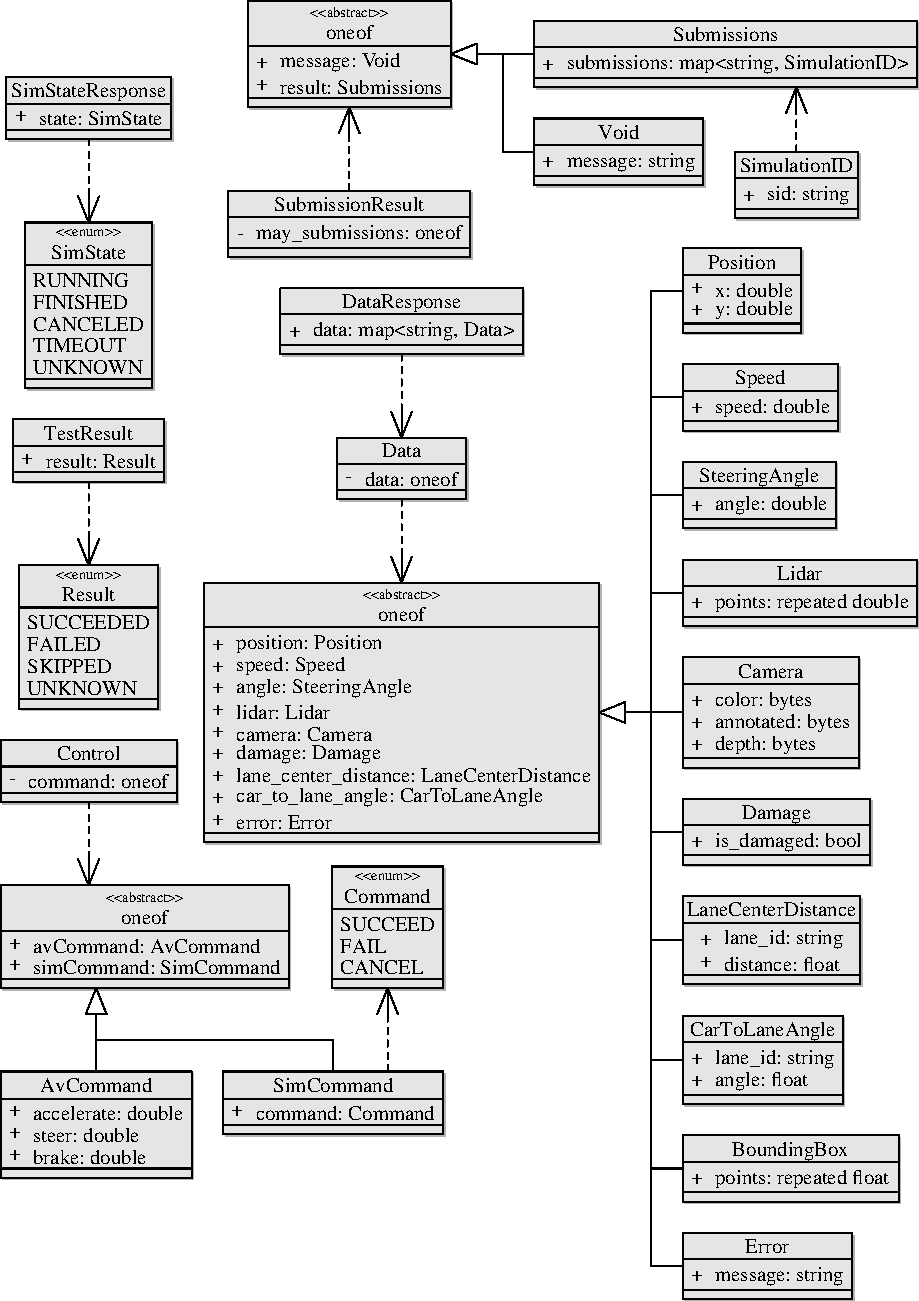
\includegraphics[width=\textwidth, height=.95\textheight, keepaspectratio]{diagrams/messagesTypeGraph-2.pdf}
    \medskip
    \caption{%
        Complex \glspl{pmessage} --- Shows the composition structure of the complex \glspl{pmessage} that \drivebuild{} can handle.
        Private attributes denote the existence and the name of exclusive groups of attributes (\code{oneof}).
    }\label{fig:complexMessages}
\end{figure}
\Glspl{pmessage} are considered as complex if they have at least one attribute whose type is either another \gls{pmessage}, an enum or an exclusive group of attributes (\code{oneof}).
An \code{oneof} group is not a \gls{pmessage} on its own but logically the superclass of multiple other \glspl{pmessage}.
\Glspl{pmessage} can only be properly instantiated from top level \glspl{pmessage}.
Each message on the socket level is a sequence of two sub-messages as shown in \cref{fig:socketMessage}.
\begin{figure}
    \centering
    \begin{sequencediagram}
    \newthread{a}{:A}
    \tikzstyle{inststyle}+=[below right=-0.82cm and 4cm of a]  % FIXME Workaround for newthread distance
    \newthread{b}{:B}
    \begin{callself}{b}{Wait for complete sub-messages}{}
        \mess{a}{content length}{b}
        \mess{a}{content}{b}
    \end{callself}
\end{sequencediagram}

    \medskip
    \caption{%
        Socket message --- Shows the sequence of sub-messages that form a complete message.
        This diagram assumes that A sends a message and B waits for receiving it.
    }\label{fig:socketMessage}
\end{figure}
The content length sub-message has a fixed length and sends the number of bytes that the actual content has.
The actual content sub-message is a \gls{pmessage} which contains the serialized content.
This way the receiver knows the length of both sub-messages and thus can determine whether it already got the complete message or it has to wait for more bytes to receive.
An action request is a sequence of socket messages which implements a function call over a socket.
\Cref{fig:actionRequest} visualizes the sequence of socket messages.
\begin{figure}
    \centering
    \begin{sequencediagram}
    \newthread{a}{:A}
    \tikzstyle{inststyle}+=[below right=-0.82cm and 5cm of a]  % FIXME Workaround for newthread distance
    \newthread{b}{:B}
    \begin{callself}{b}{Wait for complete message}{}
        \mess{a}{action}{b}
        \mess{a}{number of params N}{b}
        \mess[1]{a}{parameters 1 to N}{b}
    \end{callself}
    \begin{callself}{a}{Wait for complete message}{}
        \mess{b}{result}{a}
    \end{callself}
\end{sequencediagram}

    \medskip
    \caption{%
        Action request --- Shows the socket messages that a component A exchanges with component B if A requests an action that B provides.
        Each of these messages consists of sub-messages as described in \cref{fig:socketMessage}.
    }\label{fig:actionRequest}
\end{figure}
The first socket message sends an action that specifies which function has to be called.
The second socket message defines the number of arguments \(N\) which the sender passes to the function.
The next \(N\) socket messages are \glspl{pmessage} which contain the actual arguments.

\subsection{\texorpdfstring{\Glstext{mainapp}}{MainApp}}
The \gls{mainapp} is the central component of \drivebuild{} and offers an interface to all types of clients (see \cref{fig:systemArch}), manages \glspl{simnode} and distributes tests across them.
The interface for clients is a micro service~\cite{microServices} based webserver and \cref{tab:microServices} lists all its services.
\begin{table}
    \centering
    \caption{%
        \Glstext{mainapp} micro services --- Lists the micro services which the \gls{mainapp} provides, a short description, the required parameters and the return type in case a request is successful.
        All parameters have to be appended to an \glstext{url} as GET parameters except for underlined parameters which have to be sent as the content of a POST request.
        Italic entries add notes about parameters.
    }\label{tab:microServices}
    \medskip
    %!TEX root = ../thesis.tex
\def\tabularxcolumn#1{m{#1}}
\begin{tabularx}{.9\textwidth}{X l l}
    \toprule
    \bfseries \Glstext{url} & \bfseries Parameters (name: type) & \bfseries Return Type \\
    \midrule
    /runTests & \makecell[l]{user: User\\\underline{zip byte data}} & SubmissionResult \\
    \midrule
    /ai/waitForSimulatorRequest & \makecell[l]{sid: SimulationID\\vid: VehicleID} & SimStateResponse \\
    \midrule
    /ai/requestData & \makecell[l]{sid: SimulationID\\vid: VehicleID\\request: DataRequest} & DataResponse\\
    \midrule
    /ai/control & \makecell[l]{sid: SimulationID\\vid: VehicleID\\\underline{Control}} & Void \\
    \midrule
    /stats/getRunningSids & user: User & SubmissionResult \\
    \midrule
    /stats/<action> & \makecell[l]{\textit{At least:}\\sid: SimulationID\\\textit{Maybe further parameters}} & \textit{Depends on action} \\
    \midrule
    /sim/stop & \makecell[l]{sim: SimulationID\\result: TestResult} & Void\\
    \bottomrule
\end{tabularx}

\end{table}
The use of micro services hides and strictly separates functionality plus it allows finer granularity than other architectures like \gls{soa}.
From a testers perspective there is only the service \code{/runTests} which submits new tests to \drivebuild{} and starts them.
The tests have to be compressed into a zip file.
This call blocks until \drivebuild{} created all the resulting scenarios and started simulator instances which run all of them.
The response of this request maps the names of the submitted tests to the generated \code{SimulationID}\unskip{}s.
A tester requires this information to map \code{VehicleID}\unskip{}s that tests declare to \code{SimulationID}\unskip{}s and start the corresponding \glspl{ai}.
The interface for \glspl{ai} offers all micro services which they require to implement their interaction with the simulations (see \cref{fig:aiSimProtocol}).
A call to \code{/ai/waitForSimulatorRequest} registers an \gls{ai} for controlling a certain \gls{av} in a certain simulation.
This request blocks until either the simulation requests the registered \gls{ai} or it finishes.
The response contains the current state of the simulation to which this \gls{ai} registered to which allows to determine whether the \gls{ai} has to continue or to stop.
If an \gls{ai} continues it needs data for its computations.
A request to \code{/ai/requestData} retrieves the data of sensors which are attached to a participant or current values of properties of a participant like the current position or damage.
This data also allows to implement additional client side checks.
\code{/ai/control} enables an \gls{ai} to control \glspl{av} and simulations.
The returned message contains a status message which may be used for logging.
The interface of the \gls{mainapp} offers also micro services for researchers to collect and analyze test data.
So the micro service \code{/stats/<action>} provides an interface to query the database about currently running as well as previous tests.
Calls to this service require a \code{SimulationID} as a parameter and possibly further parameters which are specific to the concrete action.
The action \code{result} returns the test result of a simulation if any.
A request with the action \code{status} returns the state of the simulation like \ssrunning{}, \ssfinished{} or \sstimeout{}.
The trace of all data that a simulation collected can be retrieved by calling \code{/stats/trace}.
If a call specifies the optional parameter \code{VehicleID} the response contains only the collected data of the specified participant.
The request \code{/sim/stop} forces simulations to end and can be called from a tester as well as from an \gls{ai}.
This call requires a \code{SimulationID} and a parameter which defines the test result to set.
The result of this call contains a message which can be used for logging.
For debugging purposes of \drivebuild{} the \gls{mainapp} further offers the request \code{/stats/getRunningSids} which returns all IDs of simulations which a given user currently runs on any \gls{simnode}.\\
The interface for \glspl{simnode} is on the socket level and \cref{subsec:simnode} describes it in detail.
Besides the actual interface the \gls{mainapp} opens a port which \glspl{simnode} use to register themselves at the \gls{mainapp}.
When a new \gls{simnode} connects the \gls{mainapp} generates an unique ID, associates the incoming socket connection with it and returns the ID to the newly registered \gls{simnode}.

\subsection{\texorpdfstring{\Glstext{simnode}}{SimNode}}\label{subsec:simnode}
\Glspl{simnode} generate \beamng{} scenarios and run the actual test executions which include the simulations, the runtime verification, the interaction with \glspl{ai} and the collection of data.
% Interface to MainApp
The communication between \glspl{simnode} and the \gls{mainapp} is based on low level socket communication.
Therefore the \glspl{simcontroller} of the \glspl{simnode} offer the interface that \cref{tab:simNodeToMainAppInterface} lists which enables the \gls{mainapp} to manage simulations and to organize the interaction between on the one hand simulations and on the other hand testers and \glspl{ai}.
\begin{table}
    \centering
    \caption{%
        Interface to \gls{mainapp} --- Describes the interface to which the \gls{mainapp} sends action requests to access the functions of the \gls{simcontroller} of a \gls{simnode}.
        \Cref{fig:actionRequest} describes the structure of action requests.
    }\label{tab:simNodeToMainAppInterface}
    \medskip
    %!TEX root = ../thesis.tex
\def\tabularxcolumn#1{m{#1}}
\begin{tabularx}{.75\linewidth}{X l l}
    \toprule
    \bfseries Action & \bfseries Parameter Types & \bfseries Return Type \\
    \midrule
    runTests & \makecell[l]{User\\zip byte data} & SubmissionResult \\
    \midrule
    waitForSimulatorRequest & \makecell[l]{SimulationID\\VehicleID} & SimStateResponse \\
    \midrule
    control & \makecell[l]{SimulationID\\VehicleID\\Control} & Void \\
    \midrule
    requestData & \makecell[l]{SimulationID\\VehicleID\\DataRequest} & DataResponse \\
    \midrule
    stop & \makecell[l]{SimulationID\\TestResult} & Void \\
    \midrule
    runningTests & User & SubmissionResult \\
    \midrule
    requestSocket & --- & Void \\
    \bottomrule
\end{tabularx}

\end{table}
To use the interface the \gls{mainapp} has to make action requests.
The interface has many similarities to the micro services which the \gls{mainapp} offers to clients since many of the micro services are only redirections of requests to appropriate \glspl{simcontroller}.
This is the case for the actions \code{runTests}, \code{waitForSimulatorRequest}, \code{control}, \code{requestData} and \code{stop}.
The action \code{runningTests} searches for all \code{SimulationID}\unskip{}s of simulations which a given user currently runs on any \gls{simnode} and returns a map which associates test names with its \code{SimulationID}.
A call to the action \code{requestSocket} makes the requested \gls{simcontroller} open an additional socket which registers itself to the \gls{mainapp}.
The \gls{mainapp} uses this socket to open a socket for each \gls{ai} in each currently running simulation.\\
Since a \gls{simcontroller} runs multiple \beamng{} instances the corresponding runtime verification processes have to run simultaneously as well.
Further a \gls{simcontroller} has to share references to all \beamng{} instances with the corresponding runtime verification processes.
The exchange of data between processes in Python is based on serialization and results in deep copies of Python objects.
Since \beamng{} and \beamngpy{} use internally lots of sockets and Python is intentionally not able to serialize sockets neither \beamng{} nor \beamngpy{} instances can be easily shared.
So each \gls{simcontroller} offers a second interface (see \cref{tab:simNodeToSimulationInterface}) which runtime verification processes use to interact with \beamng{} instances and to evaluate criteria which require the current state of a simulation.
\begin{table}
    \centering
    \caption{%
        Interface to runtime verification processes --- Describes the interface that a runtime verification uses to interact with simulations using action requests.
        \Cref{fig:actionRequest} describes the structure of action requests.
    }\label{tab:simNodeToSimulationInterface}
    \medskip
    %!TEX root = ../thesis.tex
\def\tabularxcolumn#1{m{#1}}
\begin{tabularx}{.65\linewidth}{X l l}
    \toprule
    \bfseries Action & \bfseries Parameter Types & \bfseries Return Type \\
    \midrule
    vids & SimulationID & VehicleIDs \\
    \midrule
    isRunning & SimulationID & Bool \\
    \midrule
    pollSensors & SimulationID & Void \\
    \midrule
    verify & SimulationID & VerificationResult \\
    \midrule
    requestAiFor & \makecell[l]{SimulationID\\VehicleID} & Void \\
    \midrule
    steps & \makecell[l]{SimulationID\\Num} & Void \\
    \midrule
    stop & \makecell[l]{SimulationID\\TestResult} & Void \\
    \bottomrule
\end{tabularx}

\end{table}
A request with the action \code{vids} returns the IDs of all participants in a given simulation.
The action request \code{isRunning} determines whether a specific simulation runs.
The action \code{pollSensors} updates the cached data which \glspl{ai} can request about a simulation, the properties of any participant and their sensors.
The action request \code{verify} evaluates the test criteria based on the currently cached data and returns the evaluation result of the precondition, the success and the failure criteria.
A call to \code{requestAiFor} notifies all registered \glspl{ai} about newly available data.
This call blocks until for all \glspl{av} an \gls{ai} registered with the action \code{waitForSimulatorRequest}.
If so all the calls to \code{waitForSimulatorRequest} continue.
The action request \code{steps} makes a simulation continue for the given amount of ticks.
How much progress a simulation makes depends on the values \code{steps per second} which defines into how many ticks a second in the simulation time is divided and the \code{\gls{ai} frequency} which specifies after how many ticks of simulation another cycle in the runtime verification starts.\\
\Cref{fig:runtimeVerificationScheme} depicts the sequence of calls that implements the cycle.
\begin{figure}
    \centering
    %!TEX root = ../thesis.tex
\begin{sequencediagram}
    \newthread{simcontroller}{:Runtime Verification}
    \tikzstyle{inststyle}+=[below right=-0.82cm and 5cm of simcontroller]  % FIXME Workaround for newthread distance
    \newthread{simnode}{:\Glstext{simcontroller}}
    \begin{call}{simcontroller}{vids}{simnode}{VehicleIDs}
    \end{call}
    \begin{sdblock}{Loop cycle}{While simulation running}
        \begin{call}{simcontroller}{verify}{simnode}{VerificationResult}
        \end{call}
        \begin{call}{simcontroller}{pollSensors}{simnode}{Void}
        \end{call}
        \begin{sdblock}{For each \glstext{av}}{}
            \begin{call}{simcontroller}{requestAiFor}{simnode}{Void}
                \postlevel%
            \end{call}
        \end{sdblock}
        \prelevel\prelevel\prelevel%
        \begin{callself}{simcontroller}{Wait for control commands}{Apply control commands}
            \postlevel\postlevel%
        \end{callself}
        \begin{call}{simcontroller}{steps}{simnode}{Void}
        \end{call}
    \end{sdblock}
\end{sequencediagram}

    \medskip
    \caption{%
        Runtime verification calls --- Structures the calls of the runtime verification to the \gls{simcontroller}.
        It uses the interface which \cref{tab:simNodeToSimulationInterface} lists.
    }\label{fig:runtimeVerificationScheme}
\end{figure}
The only call before the first cycle starts requests the IDs of all participants in the simulation.
The first call within the cycle evaluates the test criteria and applies the decision tree in \cref{fig:verificationDecision} to determine the current test result.
If the test result is something else than \trunknown{} it stops the simulation and notifies all registered \glspl{ai} about it.
Otherwise the cycle continues.
In this case the runtime verification retrieves the current states and the sensor data of all \glspl{av} and updates the cached data which is available for \glspl{ai}.
The next calls notify all \glspl{ai} which control \glspl{av} that are either in the movement mode \mmautonomous{} or \mmtraining{} with \code{requestAiFor} about new data and waits for the \glspl{ai} to send control commands.
Therefore the runtime verification starts a separate process that waits until the \gls{simcontroller} got all control commands of all \glspl{ai} from the \gls{mainapp}.
The runtime verification first applies commands that control the simulation.
If these stop the simulation the runtime verification notifies all registered \glspl{ai} about it and exits.
Otherwise it applies the control commands which control \glspl{av} and calls \code{step} which makes the simulation continue for a few ticks.
Then the loop starts over again.\\
To implement the interaction between an \gls{ai} and a simulation on the client side the implementation of the \gls{ai} has to follow the scheme that \cref{fig:clientScheme} shows.
\begin{figure}
    \centering
    \plainFrame{%
    \centering
    \resizebox{!}{\pageheight}{%
        \begin{sequencediagram}
            \newthread{client}{:Client}
            \tikzstyle{inststyle}+=[below right=-0.82cm and 5cm of client]
            \newthread{drivebuild}{:MainApp}
            \begin{call}{client}{/runTests}{drivebuild}{SubmissionResult}
            \end{call}
            \begin{sdblock}{Handle AI}{For each AI in parallel}
                \begin{call}{client}{/ai/waitForSimulatorRequest}{drivebuild}{SimStateResponse}
                    \begin{callself}{drivebuild}{Wait for requestAiFor}{}
                    \end{callself}
                \end{call}
                \begin{call}{client}{/ai/requestData}{drivebuild}{DataResponse}
                \end{call}
                \begin{callself}{client}{Calculate control commands}{}
                \end{callself}
                \begin{call}{client}{/ai/control}{drivebuild}{Void}
                    \begin{callself}{drivebuild}{Apply control commands}{}
                    \end{callself}
                \end{call}
            \end{sdblock}
        \end{sequencediagram}
    }
    \subsectionBox{colorVerify!40}
}


    \medskip
    \caption{%
        Client scheme --- Depicts the basic scheme of the sequence of calls that a client has to make to implement interaction with \drivebuild{}.
        Therefore it has to use the interface which \cref{tab:microServices} lists.
    }\label{fig:clientScheme}
\end{figure}
The interaction uses the same \glspl{pmessage} as the low level socket communication uses (see \cref{subsec:communication}).
\Cref{fig:exampleMessageUsage} shows examples of how to create and read the most important \glspl{pmessage} which the client requires.
\begin{figure}[h]
    \captionsetup{type=listing}
    \newcounter{sublisting}
    \renewcommand{\thesublisting}{\alph{sublisting}}
    \begin{subfigure}{\textwidth}
    \centering
    \inputminted{python}{code/exampleMessageCreation.py}
    \caption{%
        Creation of simple messages
    }
\end{subfigure}
\begin{subfigure}{\textwidth}
    \centering
    \inputminted{python}{code/exampleMessageAccess.py}
    \caption{%
        Access to attributes of complex messages
    }
\end{subfigure}

    \medskip
    \caption{%
        Example \glspl{pmessage} --- Demonstrates the creation and usage of the fundamental \glspl{pmessage} that a client implementation requires.
    }\label{fig:exampleMessageUsage}
\end{figure}
The first call submits formalized test cases to \drivebuild{} and returns a map from the declared test names to the assigned \code{SimulationID}\unskip{}s.
The client starts for each participant in each simulation a separate process which interacts with the participant.
This process repeats a certain sequence of calls as long as the simulation which simulates the participant runs.
The first call in the sequence registers the process with \code{waitForSimulatorRequest} for the interaction with a specific participant in a certain simulation and blocks until one of the two following events occur.
The one event occurs if the participant enters one of the movement modes \mmautonomous{} or \mmtraining{} and the runtime verification calls \code{requestAiFor}.
The other event occurs if the simulation stops.
The call to \code{waitForSimulatorRequest} is the only required call.
Any other call may be omitted.
If the request returns and the simulation is not in state \ssrunning{} the interaction stops, the process may clean up memory and exit.
Otherwise the interaction continues and may request properties about participants or their sensor data.
At this point a client can collect training data for \glspl{ai}.
If a participant is in movement mode \mmautonomous{} the process can either calculate commands which handle the \gls{av} or send commands which control the simulation.
If the participant is in movement mode \mmtraining{} it can only control the simulation and the \gls{mainapp} ignores any command which controls an \gls{av}.
Then the sequence of interaction calls starts over again.\\
% Process of simulation generation and start
Internally a \gls{simnode} implements all phases of the test life cycle (see \cref{fig:testCycle}) and therefore the appropriate components of \drivebuild{} as \cref{fig:systemArch} shows.
The \transformer{} implements the input validation step.
Therefore it validates tests against the \gls{xsd} which \drivebuild{} provides.
The \generator{} and the \gls{kptransformer} implement the extraction step as well as the transformation step.
In the extraction step they use XPath to extract all information that the semantic model requires.
The actual semantic model results from the transformation step.
The \generator{} uses structs to represent the environment of a simulation.
The \gls{kptransformer} parses precondition, success and failure criteria from top to bottom and recursively creates \lambda{} expressions that abstractly represent the test criteria as Kleene and Priest logics expressions.
These \lambda{} expressions take a \beamng{} scenario as their input and can evaluate the criteria based on the current state of the scenario.
Further the \gls{kptransformer} attaches default data requests which collect data to partially reproduce a simulation without having to actually execute it again or which future work might require.
It also may attach additional sensors to participants if the evaluation of criteria requires further data.
On the one hand the \gls{simcontroller} creates and manages the simulations and the runtime verification processes and on the other organizes the interaction with the \gls{mainapp}.\\
Before starting a simulation the \gls{simcontroller} has to generate a \beamng{} scenario.
The level for the scenario is an infinitely big flat plain which is covered with grass.
A \beamng{} scenario consists of a \json{}, a prefab and a \lua{} file.
The \json{} file contains meta data about the scenario including its name, the author, a description and a reference to the prefab file.
The prefab file describes the static information about initial states of vehicles, roads, waypoints and \lua{} triggers.
The \gls{simcontroller} uses \beamngpy{} to create an initial \beamng{} scenario but further modifies it since \beamngpy{} does not provide all required features.\\
% initial states
The definition of positions of participants in the formalization corresponds to \beamng{} but the definition of orientations of participants defers.
The formalization defines orientation as \cref{fig:envCooSystem} shows.
In contrast \beamng{} defines orientation in clockwise manner and an orientation of \ang{0} makes the car head in negative y direction.
So the generator has to translate the orientation accordingly before placing participants in a \beamng{} scenario.
% roads
When adding a road it is smoothened by interpolating the points which the semantic model stores for its course with a cubic B-spline.
The interpolation sets the smoothness to \num{0} and adds additional points to ensure that the resulting course fits all points perfectly and the its shape is like expected.
The interpolation is done with \scipy{}~\cite{scipy}
The road markings in the scenario are implemented as narrow lanes which are parallel to the B-spline and just have a different texture than the actual road.
\scipy{} provides methods to calculate these parallel lines, \ie{} offset lines.
A road has a declared number of left and right lanes.
The generator creates two offset lines for the left and right side road marking (continuous white line), one offset line which separates left from right lanes (continuous double yellow line) and offset lines that separate left and right lanes from each other (dashed white line).
% waypoints
The dynamic behavior of participants is described by sequences of waypoints in the semantic model.
The generator adds for each of these waypoints corresponding \beamng{} waypoints which have the position and size as defined in the semantic model.
% LUA triggers
Further it adds \lua{} triggers for each \beamng{} waypoint.
\lua{} triggers define areas where custom \lua{} functions are executed as soon as the bounding box of a participant intersects with it or does not intersect with it anymore.
When a participant reaches a \lua{} trigger the simulation calls a custom \lua{} function which makes the participant move to the next \beamng{} waypoint.
Since these functions make a participant approach to a \beamng{} waypoint such a way that it almost touches the waypoint without intersecting it \lua{} triggers have to be slightly bigger than the underlying \beamng{} waypoint to make sure the participant intersects the \lua{} trigger.
When a participant reaches a \lua{} trigger the custom \lua{} function also applies the additional properties of the waypoints in the semantic model which includes target speeds, speed limits and changes of the movement mode.
Due to the internal implementation of \beamng{} a speed limit overrides a target speed.
If the generation of the \beamng{} scenario finished the \gls{simcontroller} starts a new \beamng{} instance, loads the scenario and starts the simulation.

\subsection{\texorpdfstring{\Glstext{dbms}}{DBMS}}
The database uses \postgresql{} since \postgresql{} is well known, well supported in many languages and provides the data type \code{SERIAL} which allows to easily and safely generate unique \code{SimulationID}\unskip{}s for tests.
\Cref{fig:databaseScheme} depicts the complete scheme which \drivebuild{} uses to store data about finished and currently running tests as well as data about properties and sensor data of all participants in any runtime verification cycle.
\begin{figure}
    \centering
    \begin{tikzpicture}
    \node[attribute] (sid) {\key{SimulationID}};
    \node[attribute, below=0.5 of sid] (environment) {Environment};
    \node[attribute, below=0.5 of environment] (criteria) {Criteria};
    \node[attribute, below=0.5 of criteria] (result) {TestResult};
    \node[attribute, below=0.5 of result] (status) {SimState};
    \node[attribute, below=0.5 of status] (started) {StartTime};
    \node[attribute, below=0.5 of started] (finished) {EndTime};
    \node[entity, right=of result] (test) {Tests};

    \node[ident relationship, right=of test] (of) {in};

    \node[weak entity, right=of of] (trace) {VerficationCycles};
    \node[attribute, above=of trace.north west, anchor=south] (tick) {\weakkey{Tick}};
    \node[attribute, above=of trace.north east, anchor=south] (cycleFinished) {EndTime};
    \node[attribute, below=of of] (vid) {\weakkey{VehicleID}};
    \node[attribute, below=of vid.south east, anchor=north] (data) {DataResponse};
    \node[attribute, above=of data.east, anchor=south west] (cycleStarted) {StartTime};

    \node[relationship, above right=1.5 and 0 of test] (submit) {submit};

    \node[entity, above=of submit] (user) {Users};
    \node[attribute, right=of user] (username) {\key{Username}};
    \node[attribute, above=0.5 of username] (password) {Password};

    \path
        (test) edge[bend right] (sid)
        (test) edge (environment)
        (test) edge (criteria)
        (test) edge (result)
        (test) edge (status)
        (test) edge (started)
        (test) edge[bend left] (finished)
        (trace) edge (data)
        (trace) edge (vid)
        (trace) edge (tick)
        (trace) edge (cycleStarted)
        (trace) edge (cycleFinished)
        (trace) edge[total] node[above] {n} (of)
        (of) edge node[above] {1} (test)
        (user) edge (username)
        (user) edge (password)
        (user) edge node[right] {0...1} (submit)
        (submit) edge node[above] {n} (test);
\end{tikzpicture}

    \medskip
    \caption{%
        Database scheme --- Depicts all the data that \drivebuild{} stores about executed and running tests and how the data relates.
    }\label{fig:databaseScheme}
\end{figure}
The table \enquote{Test} stores for each test execution the \code{SimulationID}, the current test result, the current state of the simulation and timestamps for when the execution started and finished.
Additionally it contains serialized byte strings of the \gls{dbe} and \gls{dbc} which specify the test.
% The table also stores the result of the test.
% As long as the simulation runs this value is \trunknown{}.
% If the simulation ends without timeout it set to either one of \trsucceeded{}, \trfailed{} or \trskipped{}.
% Furthermore the table contains the current state of simulations which is one of \ssrunning{}, \ssfinished{}, \sscanceled{} or \sstimeout{} and time stamps for when the simulation started and when it ended.
Each entry in \enquote{Test} references the user in \enquote{User} who submitted the test to \drivebuild{}.
Each user has an username and a password.
The table \enquote{VerficationCycles} stores all data which the runtime verification collects in each cycle.
This includes especially all properties and sensor data of any participants.
Since the properties as well as the sensor data is highly diverse and may change when more sensors are added or when the provided detail of sensor data increases it is very hard to specify a fixed static \gls{dbms} scheme.
So the collected data is stored in a single field where a serialized \code{DataResponse} object contains all the data.
Each entry additionally stores two timestamps that save the time from the start of a cycle until the call to \beamng{} for continuing the simulation.
